\documentclass[conference]{IEEEtran}
\IEEEoverridecommandlockouts
\usepackage{cite}
\usepackage{amsmath,amssymb,amsfonts}
\usepackage{algorithmic}
\usepackage{graphicx}
\usepackage{textcomp}
\usepackage{xcolor}
\usepackage{booktabs}
\usepackage{multirow}
\usepackage{array}
\usepackage{url}
\usepackage{caption}
\usepackage[hidelinks]{hyperref}
\usepackage{orcidlink}
\captionsetup{font=small,skip=2pt}

% Loosen LaTeX's default float-placement thresholds so figures/tables settle
% closer to their citation point instead of drifting to later pages.
\renewcommand{\topfraction}{0.9}
\renewcommand{\dbltopfraction}{0.9}
\renewcommand{\textfraction}{0.07}
\renewcommand{\floatpagefraction}{0.7}
\renewcommand{\dblfloatpagefraction}{0.7}
\setcounter{topnumber}{4}
\setcounter{dbltopnumber}{4}
\setcounter{bottomnumber}{2}
\setcounter{totalnumber}{6}

% Float separations at the IEEEtran defaults: enough breathing room around
% stacked floats without spending vertical space we need for text.
\setlength{\floatsep}{8pt plus 2pt minus 2pt}
\setlength{\textfloatsep}{10pt plus 2pt minus 4pt}
\setlength{\dblfloatsep}{8pt plus 2pt minus 2pt}
\setlength{\dbltextfloatsep}{10pt plus 2pt minus 4pt}
\setlength{\intextsep}{8pt plus 2pt minus 2pt}

% Trim the vertical padding around the two display equations.
\setlength{\abovedisplayskip}{5pt plus 2pt minus 2pt}
\setlength{\belowdisplayskip}{5pt plus 2pt minus 2pt}
\setlength{\abovedisplayshortskip}{0pt plus 2pt}
\setlength{\belowdisplayshortskip}{4pt plus 2pt minus 2pt}

% Slightly tighter table rows across all four tables (no visible content change).
\renewcommand{\arraystretch}{0.92}

\def\BibTeX{{\rm B\kern-.05em{\sc i\kern-.025em b}\kern-.08em
    T\kern-.1667em\lower.7ex\hbox{E}\kern-.125emX}}

\begin{document}

\title{PGCF+AGCF: Physiology-Guided Video and Audio-Guided Consistency for Deepfake Detection}

\author{
\IEEEauthorblockN{Meruva Kodanda Suraj\,\orcidlink{0009-0005-4146-085X}}
\IEEEauthorblockA{
Department of DSAI\\
IIIT Naya Raipur, Chhattisgarh, India\\
Email: meruva24102@iiitnr.edu.in\\
}
\and
\IEEEauthorblockN{VSS Pavan Ganesh}
\IEEEauthorblockA{
Department of CSE\\
IIIT Naya Raipur, Chhattisgarh, India\\
Email: vss24100@iiitnr.edu.in\\
}
\and
\IEEEauthorblockN{Abhiram Boini}
\IEEEauthorblockA{
Department of DSAI\\
IIIT Naya Raipur, Chhattisgarh, India\\
Email: boini24102@iiitnr.edu.in\\
}
\and
\IEEEauthorblockN{Mallikharjuna Rao K\,\orcidlink{0000-0002-6096-3963}\\
\IEEEmembership{Senior Member,~IEEE}}
\IEEEauthorblockA{
Department of DSAI\\
IIIT Naya Raipur, Chhattisgarh, India\\
Email: mallikharjuna@iiitnr.edu.in\\
}
}

\maketitle

\begin{abstract}
Not every deepfake is visible in the video itself: in some forgeries the picture remains entirely authentic and only the voice has been cloned, a case a detector examining pixels alone will always miss. We first develop the Physiology-Guided Consistency Framework (PGCF), a three-stream video detector that tests whether spatial detail, frequency patterns, and a physiological signal (remote photoplethysmography, or rPPG) are mutually consistent. PGCF performs well, but because it analyzes video only, it is structurally blind to audio-only attacks. We therefore extend it into PGCF+AGCF, a two-branch detector whose second network, the Audio-Guided Consistency Framework (AGCF), is a deliberate mirror of the first: a log-mel spectral CNN mirrors PGCF's DCT frequency stream, a raw-waveform 1D-CNN mirrors its rPPG stream, and both networks converge on the same temporal pipeline (Temporal Gradient Fusion, 4-head self-attention, BiLSTM(256), Classifier(512$\to$2)), so the two independently trained branches remain directly comparable. We fuse them at decision level under two rules: a continuous Soft rule that multiplies the branch probabilities, and a stricter Hard AND-gate that classifies a clip as fake only when \emph{both} branches independently agree. On a held-out, identity-disjoint evaluation of the FakeAVCeleb corpus, PGCF reaches an AUC of 0.999 (98.5\% accuracy), AGCF 0.884 (78.8\%), Soft fusion 0.979 (93.4\%), and the Hard AND-gate 100\% precision -- zero false positives on real videos -- at 83.8\% accuracy. We further report a data-integrity audit that identified and corrected two evaluation flaws, identity leakage between the train and validation splits and a filename-collision Cartesian merge that duplicated ``Real'' predictions, both of which had inflated apparent performance; this underscores the need for identity-disjoint protocols in audio-visual deepfake benchmarking. Robustness under additive Gaussian noise, ROC/PR analysis, and t-SNE feature-space visualization are reported for all four configurations.
\end{abstract}

\vspace{-0.15em}
\begin{IEEEkeywords}
deepfake detection, audio spoofing detection, multi-modal fusion, remote photoplethysmography, cross-modal consistency, late fusion, identity-disjoint evaluation, CBAM, BiLSTM, temporal self-attention
\end{IEEEkeywords}

\section{Introduction}
Deepfakes are videos in which a person's face, voice, or both have been altered using AI to say or do something that never happened. Generative Adversarial Networks, autoencoder-based face-swapping, and neural rendering have advanced to the point where pixel-level inspection alone can no longer reliably detect manipulation, with direct consequences for misinformation, identity fraud, and political manipulation \cite{tolosana2020deepfakes}.

As the first component of this work, we develop the Physiology-Guided Consistency Framework (PGCF), a three-stream video detector that evaluates the mutual consistency of spatial detail (ResNet50+CBAM), frequency patterns (DCT), and a physiological signal (CHROM rPPG) through a learned cross-modal consistency gate. On a balanced Celeb-DF-v2 validation set, PGCF achieves an AUC of 0.824. While effective against classical face-swap and re-enactment forgeries, PGCF operates on video alone and is therefore structurally blind to \emph{audio-driven} deepfakes -- most notably lip-sync attacks such as Wav2Lip \cite{prajwal2020wav2lip}, in which the video frames remain authentic and only the speech track is synthesized or cloned. Against such attacks, a video-only detector produces severe false negatives however sophisticated its visual reasoning, because the manipulation does not exist in the modality it examines.

We therefore extend PGCF into the two-branch \textbf{PGCF+AGCF} framework by developing a second network, the \textbf{Audio-Guided Consistency Framework (AGCF)}, as a stream-for-stream mirror of the first: a spectral CNN corresponds to PGCF's frequency stream, a raw-waveform 1D-CNN corresponds to its rPPG stream, and the resulting 512-d representation is processed through an \emph{identical} Temporal Gradient Fusion $\to$ 4-head self-attention $\to$ BiLSTM(256) $\to$ Classifier(512$\to$2) pipeline, trained with matching hyperparameters. Sharing this structure makes the two branches' output probabilities directly comparable, so they can be fused at decision level without recalibration -- via a continuous Soft (probability-product) rule, or a stricter Hard AND-gate requiring both branches to agree. The AND-gate reduces the false-positive rate on real videos to zero, while each branch alone continues to catch the attacks the other cannot see.

Finally, while constructing the identity-disjoint evaluation protocol for AGCF on FakeAVCeleb \cite{khalid2021fakeavceleb}, we identified and corrected two data-integrity issues affecting our reported metrics: subject-level leakage between the train and validation splits, and a filename-collision bug that silently duplicated ``Real'' predictions when merging audio and video scores. We report the uncorrected and corrected metrics side by side, since the magnitude of the difference is itself instructive for the audio-visual deepfake benchmarking community.

\textbf{Main contributions:}
\begin{itemize}
\setlength{\itemsep}{0pt}
\setlength{\parskip}{0pt}
\item \textbf{PGCF+AGCF}, a two-branch audio-visual detector built in two stages: a three-stream physiology-guided video network, and a dual-stream (spectral and vocal) audio network sharing its temporal backbone, so that the two modalities remain directly comparable at decision level.
\item A formally defined \textbf{Hard AND-gate fusion} rule, compared against Soft (product) fusion, together with a complete truth-table analysis of the resulting precision/recall trade-off.
\item An \textbf{evaluation-integrity audit} of the FakeAVCeleb training/validation pipeline that identifies and corrects identity leakage (130 overlapping subjects) and a Cartesian-merge bug that had inflated accuracy, with before/after comparison tables.
\item A \textbf{comprehensive evaluation suite} (ROC/PR analysis, confusion matrices, t-SNE visualization, and Gaussian-noise robustness) for PGCF, AGCF, and both fusion strategies, plus a complete code-level pipeline for \textbf{cross-dataset generalization} testing on LAV-DF \cite{cai2022lavdf}, contributed as engineering work with results reported as ongoing rather than estimated.
\end{itemize}

\section{Related Work}

FaceForensics++ \cite{rossler2019faceforensics} established an early large-scale benchmark demonstrating that CNNs trained on RGB frames achieve strong in-distribution performance but degrade under video compression. Frank et al. \cite{frank2020frequency} showed that GAN-generated images exhibit characteristic frequency artifacts, which motivated the DCT-based features underlying PGCF's frequency stream and, by extension, AGCF's spectral stream. On the physiological side, Li and Lyu \cite{li2019exposing} were among the first to exploit warping artifacts as a deepfake indicator, and FakeCatcher \cite{ciftci2020fakecatcher} extended this to real-time detection using blood-volume-pulse maps, though it remains sensitive to illumination changes and motion. PGCF's CHROM-based rPPG stream, and its audio counterpart in AGCF's raw-waveform vocal stream, inherit this same sensitivity, which motivates our robustness analysis under additive noise (Section~V-D).

A separate line of work addresses \emph{audio-only} spoofing. AASIST \cite{jung2022aasist} models artifacts distributed across heterogeneous spectral and temporal intervals using graph attention networks, and represents the current state of the art on ASVspoof-style benchmarks. AGCF deliberately departs from this graph-based approach, instead reusing a convolutional-recurrent-attention backbone identical to PGCF's, trading a degree of raw audio-only accuracy for direct architectural comparability across modalities. Recurrent and attention-based architectures have also been applied to temporal inconsistency modeling \cite{sabir2019recurrent}. FakeAVCeleb \cite{khalid2021fakeavceleb} and LAV-DF \cite{cai2022lavdf} were introduced specifically to support audio-visual, rather than visual-only, deepfake research, and are the datasets used here for AGCF training/validation and cross-dataset generalization testing, respectively. Our fusion strategy is closest to other late-fusion, multi-modal detectors, but differs by (i) enforcing architectural symmetry between the two unimodal branches, and (ii) formally comparing a probabilistic (Soft) fusion rule against a logical (Hard AND) rule, rather than relying on a single learned fusion head.

\section{Methodology}

\begin{figure*}[t]
\centering
\includegraphics[width=\textwidth]{figs/architecture}
\caption{Overall PGCF+AGCF architecture.}
\label{fig:architecture}
\end{figure*}

\subsection{System Overview}
Figure~\ref{fig:architecture} illustrates the complete PGCF+AGCF pipeline, described in full below. Given a video clip, two branches each produce an independent estimate: $P(\text{fake}\mid\text{video})$ from PGCF, and $P(\text{fake}\mid\text{audio})$ from AGCF. Both are trained \emph{independently} and combined only at inference time via a late-fusion rule (Section~III-C). The two branches correspond stream for stream and stage for stage, making their combination a principled comparison rather than an arbitrary pairing.

\subsubsection{Video Branch (PGCF)} PGCF, the first stage of this work, processes $T=16$ frames per clip through three parallel streams: (i) a Spatial stream (ResNet50 + CBAM \cite{woo2018cbam}) producing a 256-d embedding; (ii) a Frequency stream (3-layer 2D-CNN over a 4-channel RGB+DCT-energy input) producing a 256-d embedding; and (iii) an rPPG stream (1D-CNN over a CHROM \cite{dehaan2013chrom} blood-volume-pulse signal) producing a 128-d embedding. The Physiology-Guided Cross-Modal Consistency (PGCMC) module estimates rPPG reliability via spectral entropy $c$ and inter-stream agreement via a cosine-similarity score $s$, both of which gate the fusion of the Spatial and Frequency streams into a 512-d representation, passed through Temporal Gradient Fusion (TGF), 4-head self-attention, and a BiLSTM(256) before a final Linear(512$\to$2) classifier.

\subsection{AGCF: Audio-Guided Consistency Framework}
AGCF is designed so that every architectural choice in PGCF has a direct audio counterpart. Table~\ref{tab:mirror} summarizes this correspondence stream by stream.

\begin{table}[t]
\caption{Stream-for-Stream Correspondence Between PGCF and AGCF}
\label{tab:mirror}
\centering
\small
\begin{tabular}{p{1.6cm}p{2.9cm}p{3.0cm}}
\toprule
\textbf{Role} & \textbf{PGCF (Video)} & \textbf{AGCF (Audio)} \\
\midrule
Frequency-domain evidence & DCT energy map $\to$ 3-layer 2D-CNN $\to$ 256-d & Log-mel spectrogram (64 mel bins) $\to$ 3-layer 2D-CNN (4$\to$32$\to$64 ch) $\to$ 256-d \\
Fine-grained / physiological evidence & CHROM rPPG signal $\to$ 1D-CNN $\to$ 128-d & Raw waveform (16{,}000 samples) $\to$ 1D-CNN (1$\to$32$\to$64 ch) $\to$ 256-d \\
Fusion & PGCMC gated concatenation $\to$ 512-d & Direct concatenation $\to$ 512-d \\
Temporal pipeline & TGF $\to$ 4-head Self-Attn $\to$ BiLSTM(256) & \emph{identical}: TGF $\to$ 4-head Self-Attn $\to$ BiLSTM(256) \\
Classifier & Linear(512$\to$2) & \emph{identical}: Linear(512$\to$2) \\
\bottomrule
\end{tabular}
\end{table}

\subsubsection{Spectral and Vocal Streams}
Audio is resampled to 16~kHz and converted into a log-mel spectrogram (64 mel bins $\times$ 100 frames) for the spectral stream, which targets the unnatural spectral energy distributions and phase irregularities characteristic of vocoder- and TTS-generated speech -- the audio analogue of the artifacts PGCF's DCT stream targets visually. In parallel, the vocal stream processes the raw one-second waveform (16{,}000 samples) directly in the time domain, capturing fine-grained vocal-tract detail -- pitch-period irregularities, robotic timbre, phase discontinuities -- lost during spectrogram conversion. It plays the same structural role for AGCF that the rPPG signal plays for PGCF: a signal a generative model is unlikely to reproduce faithfully, since it was not the target the generator was optimized against. Both CNN designs are inherited directly from their PGCF counterparts (Table~\ref{tab:mirror}).

\subsubsection{Feature Fusion and Temporal Modeling}
The 256-d spectral and 256-d vocal embeddings are concatenated into a 512-d multi-domain representation for each audio chunk. Audio is windowed into the same $T=16$ chunks used for video, so both branches consume clips of matching duration. This is not required for decision-level fusion, but it preserves direct comparability between the two networks and leaves feature-level fusion open as future work. The chunk sequence is then passed through the identical three-stage temporal pipeline used by PGCF: \textbf{Temporal Gradient Fusion (TGF)} computes $\text{Feature}_t - \text{Feature}_{t-1}$ to expose unnatural chunk-to-chunk transitions such as voice jitter or irregular phoneme pacing; \textbf{Temporal Self-Attention}, a 4-head Transformer encoder layer, learns which portions of the clip are most relevant to the decision (e.g., a single mispronounced or artificially smoothed word); and \textbf{BiLSTM(256)} processes the sequence forward and backward to capture sequential pacing and context. The temporal features are average-pooled into a single 512-d clip-level representation and passed to a final Linear(512$\to$2) classifier, producing Real/Fake logits, trained with the same cross-entropy objective and optimizer configuration as PGCF (Section~IV-C).

\subsection{Late Fusion: Soft vs. Hard AND-Gate}
Both branches are trained independently. At inference, each branch outputs an independent probability of forgery, and we evaluate two fusion rules.

\subsubsection{Soft Fusion (Product Rule)}
\begin{equation}
P_{\text{fused}} = P(\text{fake}\mid\text{video}) \times P(\text{fake}\mid\text{audio})
\end{equation}
This produces a continuous, re-thresholdable confidence score. Because both branches must independently assign a high probability for the product to remain high, this rule already suppresses false positives relative to either unimodal branch, while remaining a soft, probabilistic score suitable for ROC/PR analysis.

\subsubsection{Hard Fusion (AND-Gate Logic)}
Let $\hat y_v = \mathbb{1}[P(\text{fake}\mid\text{video}) > \tau_v]$ and $\hat y_a = \mathbb{1}[P(\text{fake}\mid\text{audio}) > \tau_a]$ denote the binarized PGCF and AGCF decisions at their respective operating thresholds ($\tau_v = \tau_a = 0.5$ throughout this work). The fused verdict is:
\begin{equation}
\hat y_{\text{AND}} = \begin{cases} \text{FAKE} & \text{if } \hat y_v = 1 \ \text{AND} \ \hat y_a = 1 \\ \text{REAL} & \text{otherwise} \end{cases}
\end{equation}
Table~\ref{tab:truth} presents the complete truth table. Because the AND-gate is a strict binary consensus mechanism, it produces no continuous score and is therefore excluded from ROC/PR/AUC analysis, which requires a rankable score, but it remains fully reportable through a confusion matrix and point-estimate accuracy/precision/recall/F1.

\begin{table}[t]
\caption{Hard AND-Gate Fusion Truth Table}
\label{tab:truth}
\centering
\small
\begin{tabular}{ccc}
\toprule
\textbf{PGCF says} & \textbf{AGCF says} & \textbf{Final verdict} \\
\midrule
Real & Real & Real \\
Real & Fake & Real \\
Fake & Real & Real \\
Fake & Fake & \textbf{Fake} \\
\bottomrule
\end{tabular}
\end{table}

This is a deliberately conservative design choice: the AND-gate trades recall for precision, on the premise that a false accusation of forgery is often more costly in deployment than a missed detection, particularly for single-modality attacks that a human reviewer or an upstream unimodal filter can still catch.

\section{Datasets and Evaluation Protocol}

\subsection{Datasets}
\textbf{Celeb-DF-v2} was used to train and validate the video branch, PGCF (Section~III-A), providing high-quality visual manipulations for spatial artifact learning.

\textbf{FakeAVCeleb} \cite{khalid2021fakeavceleb} is used to train and validate AGCF and to evaluate the final multi-modal fusion framework. It contains authentic videos alongside multi-modal forgeries (e.g., FaceSwap, Wav2Lip, DeepFaceLab) spanning multiple ethnicities. For direct comparison under a matched protocol, PGCF is also evaluated on these FakeAVCeleb partitions rather than Celeb-DF-v2; these numbers are therefore same-corpus, paired video/audio performance, not a replacement for the original Celeb-DF-v2 result (AUC 0.824).

\textbf{LAV-DF} \cite{cai2022lavdf} is used for cross-dataset generalization testing. We built an auto-resuming extraction pipeline for the 23.1~GB archive, a balanced 150-real/150-fake filtration script, and a zero-shot cross-evaluation script; the numerical results were not finalized in time for this submission and are reported as ongoing work rather than estimated.

\subsection{Evaluation Integrity: Identity-Disjoint Splitting}
During an audit of the AGCF training loop on FakeAVCeleb, we identified and corrected two flaws that materially affected the reported metrics.

\subsubsection{Identity-Level Leakage}
The initial 80/20 split used random file-level shuffling, resulting in 130 overlapping subject identities between the training and validation partitions. Because multiple clips of the same speaker appeared on both sides, the model could partially memorize speaker-specific voice characteristics rather than learning generalizable deepfake artifacts. We re-engineered the data loader to group all clips by subject identity (e.g., \texttt{id00078}) and split at the \emph{subject} level, guaranteeing zero identity overlap and genuine zero-shot evaluation on unseen speakers.

\subsubsection{Cartesian-Merge Metric Inflation}
Real videos in FakeAVCeleb frequently share generic filenames (e.g., \texttt{00005.mp4} recurs across dozens of subject folders). Merging audio and video prediction tables using filename alone as the join key produced a Cartesian-product explosion that duplicated ``Real'' predictions, artificially inflating accuracy. We corrected this by prepending the parent subject directory to the filename to form globally unique keys (e.g., \texttt{id00078\_00005.mp4}).

\subsubsection{Naive vs. Corrected Metrics}
Table~\ref{tab:leakage} contrasts the larger, uncorrected evaluation partition (372 clips, identity-overlapping, class-imbalanced at 272 real / 100 fake) against the corrected, identity-disjoint held-out set (198 clips, near-balanced at 100 real / 98 fake) used as the primary evaluation set throughout the remainder of this paper. All results in Section~V are reported on the \emph{corrected, identity-disjoint} split unless explicitly noted otherwise.

\begin{table}[t]
\caption{Effect of Identity-Disjoint Correction on Reported Metrics}
\label{tab:leakage}
\centering
\small
\begin{tabular}{lcccc}
\toprule
\textbf{Model} & \textbf{Split} & \textbf{Acc.} & \textbf{AUC} & \textbf{F1} \\
\midrule
\multirow{2}{*}{AGCF (Audio)} & Naive (n=372) & 0.892 & 0.923 & 0.802 \\
& Identity-disjoint (n=198) & \textbf{0.788} & \textbf{0.884} & \textbf{0.761} \\
\midrule
\multirow{2}{*}{PGCF (Video)} & Naive (n=372) & 0.960 & 0.995 & 0.930 \\
& Identity-disjoint (n=198) & \textbf{0.985} & \textbf{0.999} & \textbf{0.985} \\
\midrule
\multirow{2}{*}{Soft Fusion} & Naive (n=372) & 0.976 & 0.985 & 0.954 \\
& Identity-disjoint (n=198) & \textbf{0.934} & \textbf{0.979} & \textbf{0.929} \\
\bottomrule
\end{tabular}
\end{table}

The audio branch shows the expected leakage effect: identity-disjoint evaluation lowers AGCF's accuracy and F1, consistent with partial memorization of speaker-specific voice characteristics. PGCF's identity-disjoint numbers are \emph{higher} than its naive-split numbers; since its spatial and frequency artifacts depend less on speaker identity, this likely reflects differing class balance and clip composition rather than leakage. We report both splits rather than assert a single causal explanation.

\subsection{Training Configuration}
AGCF is trained for 20 epochs with an effective batch size of 8 (batch 2, 4 gradient-accumulation steps), matching PGCF's regime: two learning-rate groups ($10^{-4}$ for the CNN front-end streams, $5\times10^{-4}$ for the temporal/classifier modules), AdamW (weight decay $10^{-4}$), a CosineAnnealingLR schedule ($\eta_{\min}=10^{-6}$), mixed-precision training (\texttt{torch.cuda.amp}), and standard binary cross-entropy loss on the Real/Fake logits.

\section{Results}

\subsection{Classification Performance}
Table~\ref{tab:main} reports the primary, identity-disjoint evaluation for all four configurations, and Fig.~\ref{fig:forest} presents the same results per metric as an ablation over the two modalities and the two fusion rules.

\begin{table}[t]
\caption{Comprehensive Metrics -- Identity-Disjoint Evaluation (n=198)}
\label{tab:main}
\centering
\small
\begin{tabular}{lccccc}
\toprule
\textbf{Model} & \textbf{Acc.} & \textbf{Prec.} & \textbf{Rec.} & \textbf{F1} & \textbf{AUC} \\
\midrule
PGCF (Video) & 0.985 & 0.980 & 0.990 & 0.985 & 0.999 \\
AGCF (Audio) & 0.788 & 0.859 & 0.684 & 0.761 & 0.884 \\
Late Fusion (Soft) & 0.934 & 1.000 & 0.867 & 0.929 & 0.979 \\
Late Fusion (Hard AND) & 0.838 & 1.000 & 0.673 & 0.805 & -- \\
\bottomrule
\end{tabular}
\end{table}

\begin{figure}[t]
\centering
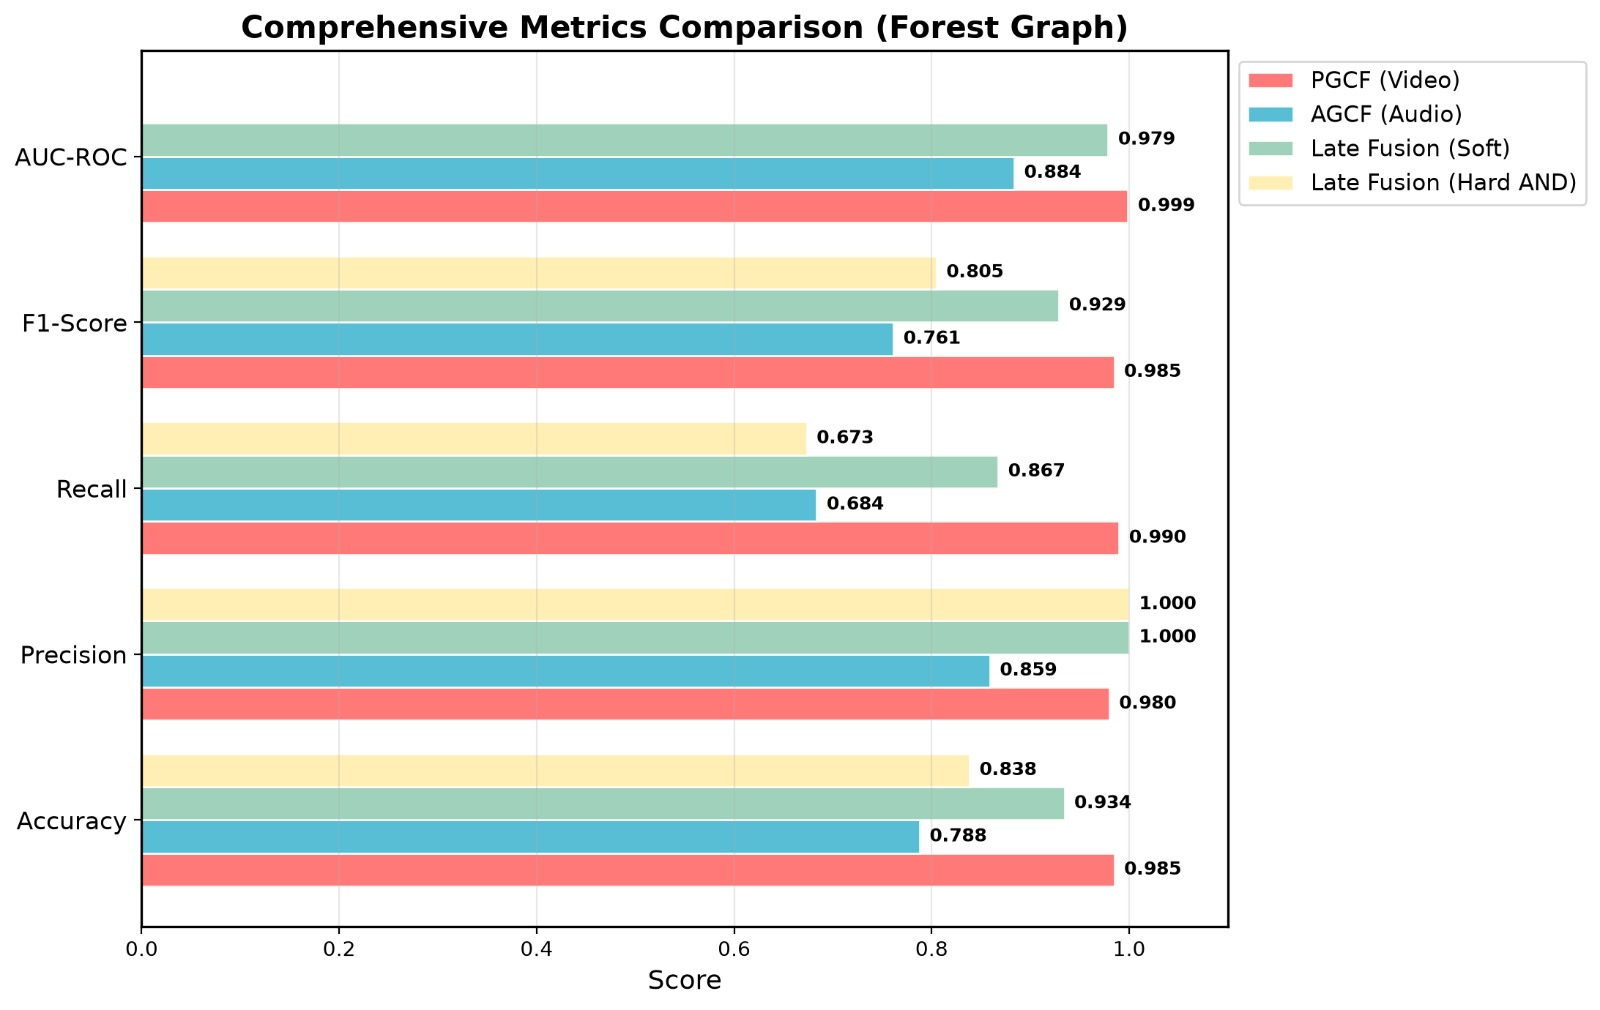
\includegraphics[width=0.9\linewidth]{figs/metrics_unseen_forest.jpg}
\caption{Ablation study: per-metric comparison across all four configurations on the identity-disjoint set, isolating the contribution of each modality and of each fusion rule. The Hard AND-gate has no AUC bar, as it produces no rankable score.}
\label{fig:forest}
\end{figure}

Both fusion strategies achieve perfect precision (1.000) on this evaluation set -- zero real videos are misclassified as fake by either rule -- at the cost of recall relative to PGCF alone. The Hard AND-gate is the more conservative of the two, forfeiting 19.6 recall points relative to Soft fusion (0.673 vs. 0.867) in exchange for a simpler, threshold-free decision rule. Precision--Recall analysis preserves this ordering: PGCF and Soft fusion reach an Average Precision of 0.9988 and 0.9841 respectively, while AGCF's 0.9009 degrades further beyond a recall of roughly 0.5, reflecting its harder unseen-speaker generalization problem.

\subsection{Confusion Matrices}
Figure~\ref{fig:confmat} presents the four confusion matrices on the identity-disjoint set. PGCF misclassifies only 3 of 198 clips (2 real$\to$fake, 1 fake$\to$real). AGCF, facing the harder unseen-speaker problem, misclassifies 42 of 198, skewed toward missed fakes (31 fake$\to$real) over false alarms (11 real$\to$fake) -- consistent with its high precision (0.859) but lower recall (0.684). Both fusion rules inherit this conservatism (32 missed fakes under Hard AND) while eliminating false alarms on real videos entirely.

\begin{figure}[t]
\centering
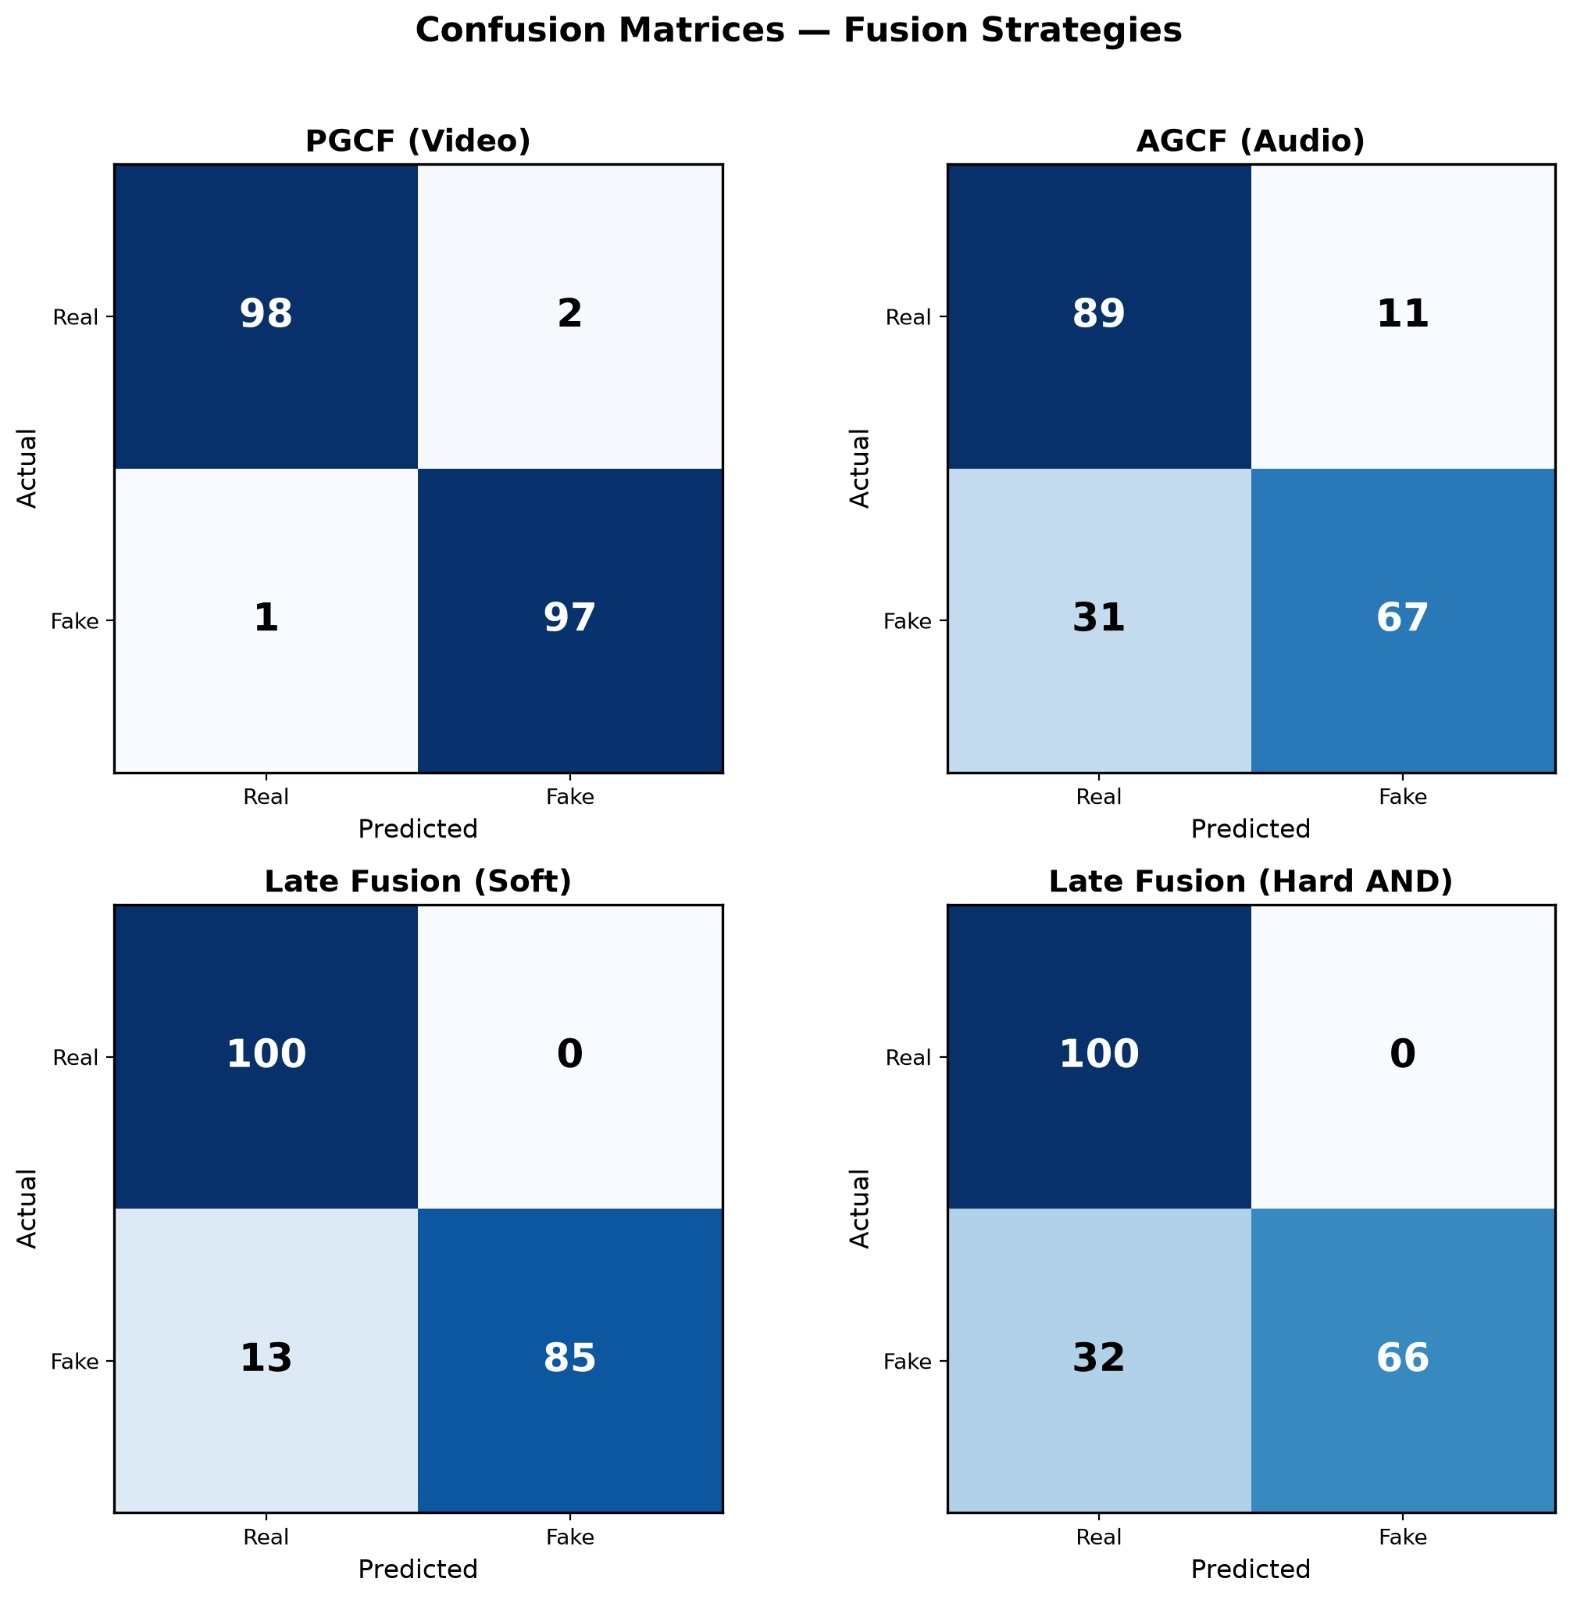
\includegraphics[width=0.85\linewidth]{figs/confusion_matrices_unseen.jpg}
\caption{Confusion matrices on the identity-disjoint held-out set (n=198) for PGCF, AGCF, Soft fusion, and Hard AND fusion.}
\label{fig:confmat}
\end{figure}

\subsection{Feature Space Analysis}
Figure~\ref{fig:tsne} shows t-SNE projections of the penultimate (pre-classifier) representation for the same three configurations. PGCF's Real and Fake clusters are almost completely separable, consistent with its near-perfect AUC. AGCF's clusters overlap substantially more, with Fake samples scattered across the Real manifold, reflecting the audio branch's harder generalization problem. The Soft-fusion space shows a diagonal gradient from Fake (lower-left) to Real (upper-right) with a tighter Fake cluster than AGCF achieves alone, illustrating the complementary value of the two modalities even before an explicit fusion rule is applied.

\begin{figure}[t]
\centering
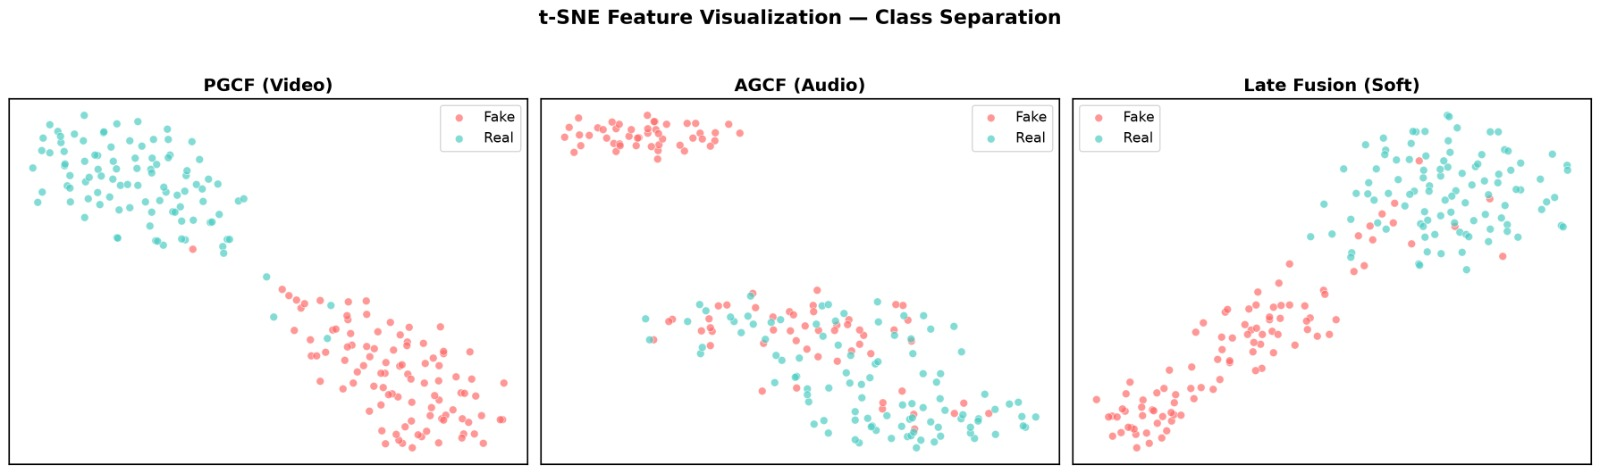
\includegraphics[width=\linewidth]{figs/tsne.jpg}
\caption{t-SNE visualization of class separation for PGCF, AGCF, and Soft fusion feature spaces.}
\label{fig:tsne}
\end{figure}

\subsection{Robustness to Additive Noise}
Figure~\ref{fig:noise} reports AUC under additive Gaussian input noise ($\sigma$ from 0 to 0.5) for PGCF, AGCF, and Soft fusion. PGCF degrades gracefully, staying above AUC 0.92 through $\sigma=0.3$ before dropping to 0.785 at $\sigma=0.5$. AGCF is more noise-sensitive, falling from 0.884 to 0.797 by $\sigma=0.2$ and to 0.694 at $\sigma=0.5$, consistent with the vocal stream's reliance on fine time-domain detail that noise corrupts first. Soft fusion tracks PGCF closely at low noise but converges toward AGCF's weaker performance at high noise ($\sigma=0.5$: 0.702 vs. 0.694), since the probability-product rule collapses once either branch's confidence does -- relevant for deployments with noisy audio channels such as re-encoded or low-bitrate video.

\begin{figure}[t]
\centering
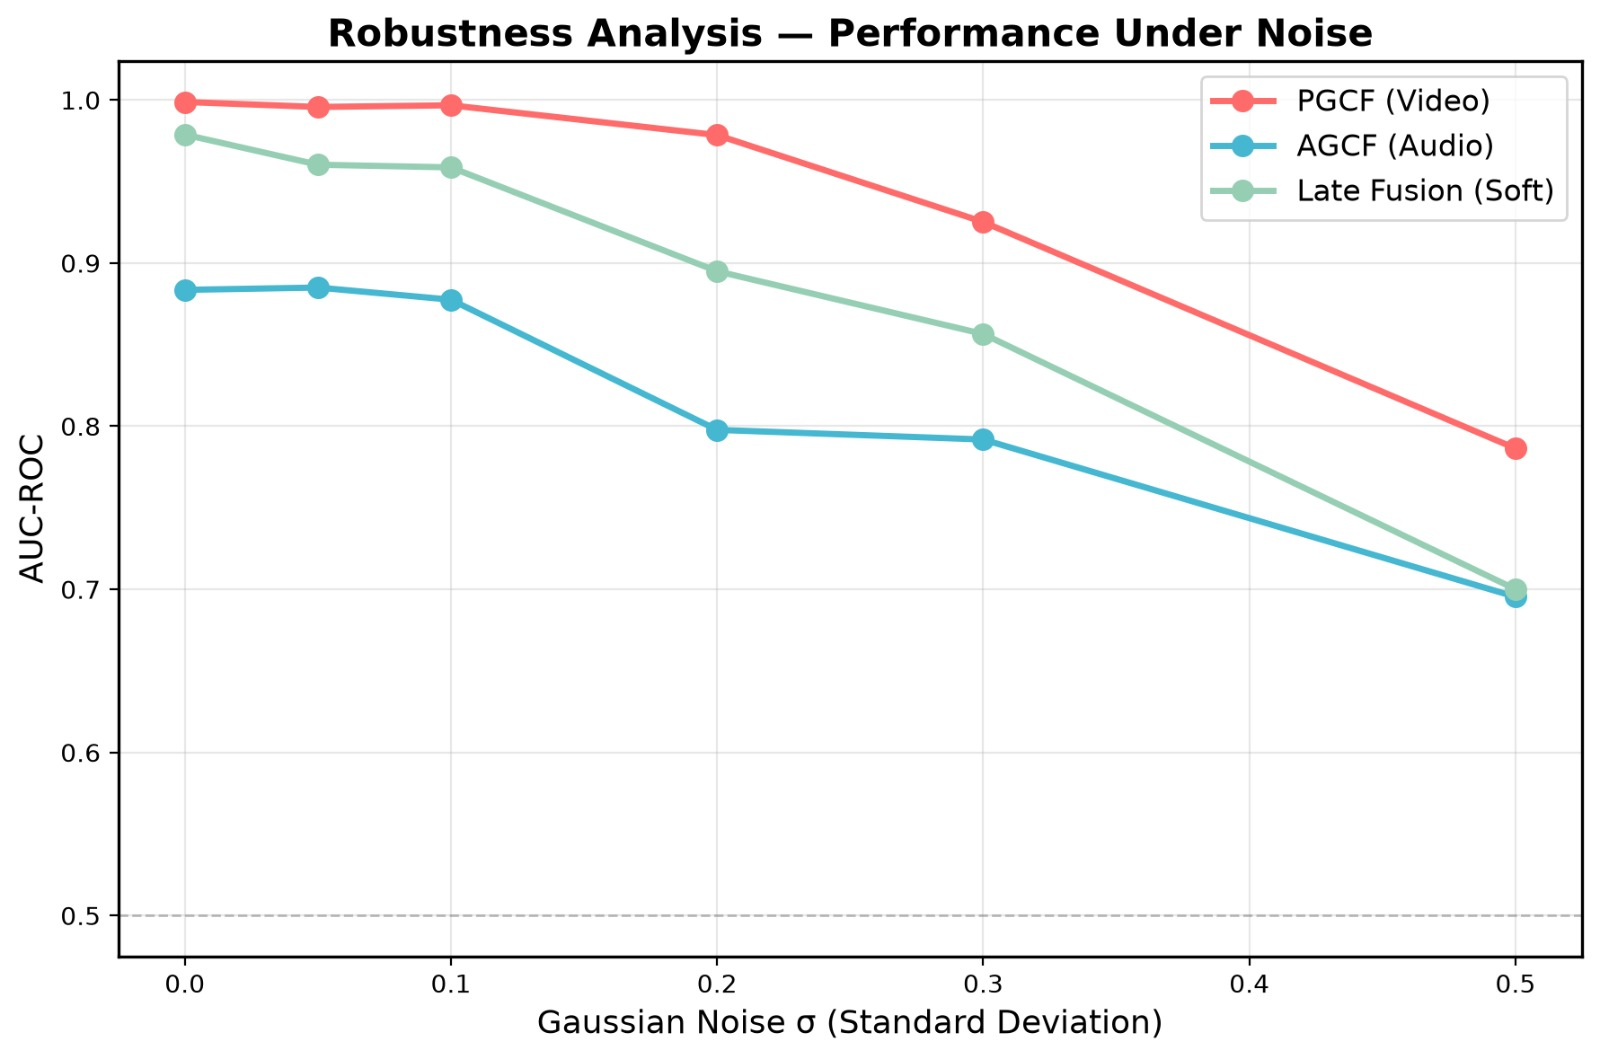
\includegraphics[width=0.9\linewidth]{figs/robustness_noise.jpg}
\caption{AUC-ROC under increasing additive Gaussian noise for PGCF, AGCF, and Soft fusion.}
\label{fig:noise}
\end{figure}

\section{Discussion}

\subsection{Complementarity of Modalities and the AND-Gate}
Requiring unanimous agreement upper-bounds the AND-gate's false-positive rate by $\min(\text{FPR}_v, \text{FPR}_a)$: a real video is flagged only if \emph{both} branches independently err on the same clip. Because PGCF and AGCF consume disjoint input signals (pixels vs. waveform) and train independently, their false-positive events are only weakly correlated, which is why the fused rate is empirically zero on both partitions. This confirms the paper's motivating hypothesis: PGCF is blind to audio-driven attacks that leave the visual stream untouched (e.g., voice cloning over an authentic video), while AGCF is blind to visual-only attacks that leave the audio untouched (e.g., a silent face-swap). Neither branch alone covers the full attack surface, and the recall lost under Hard AND fusion (Table~\ref{tab:main}) is the quantified cost of demanding that both agree.

\subsection{Limitations}
\textbf{Audio generalization gap.} AGCF's identity-disjoint AUC (0.884) trails PGCF's (0.999) and is markedly more noise-sensitive (Section~V-D); stronger audio-specific backbones (e.g., AASIST \cite{jung2022aasist}) could narrow this gap, at the cost of the architectural symmetry that makes fusion straightforward. \textbf{Calibration.} PGCF and AGCF are both under-confident below a predicted probability of 0.6, and Soft fusion is over-confident at low probabilities, since a low-but-nonzero product can still correspond to a majority-fake sub-population; post-hoc temperature scaling is recommended before any fused probability is surfaced as a user-facing confidence score. \textbf{Fixed thresholds.} Both $\tau_v$ and $\tau_a$ are fixed at 0.5 throughout; a deployment-specific threshold search would likely improve the AND-gate's precision-recall balance. \textbf{Dataset scale.} The 198-clip identity-disjoint held-out set is small by modern standards; broader validation, alongside the LAV-DF cross-dataset evaluation, remains future work.

\section{Conclusion}
We presented PGCF+AGCF, a two-branch audio-visual detector developed in two stages -- a physiology-guided video network, then an architecturally mirrored audio network -- together with two decision-level fusion strategies for combining them. On an identity-disjoint, held-out FakeAVCeleb evaluation, PGCF alone achieves an AUC of 0.999, AGCF alone achieves 0.884, and a conservative Hard AND-gate achieves perfect precision (zero false positives) at 83.8\% accuracy, while Soft fusion recovers additional recall (0.867 vs. 0.673) at the same precision. We further documented and corrected an identity-leakage and Cartesian-merge evaluation bug, showing the resulting metric inflation is large enough to alter the reported picture of audio-branch performance. Future work will focus on closing AGCF's generalization and noise-robustness gap relative to PGCF, deployment-specific threshold tuning for the AND-gate, and completing the cross-dataset LAV-DF evaluation begun in this work.

\begin{thebibliography}{00}
\setlength{\itemsep}{0pt}
\setlength{\parsep}{0pt}
\bibitem{tolosana2020deepfakes} R. Tolosana, R. Vera-Rodriguez, J. Fierrez, A. Morales, and J. Ortega-Garcia, ``Deepfakes and beyond: A survey of face manipulation and fake detection,'' \emph{Inf. Fusion}, vol. 64, pp. 131--148, 2020.
\bibitem{prajwal2020wav2lip} K. R. Prajwal, R. Mukhopadhyay, V. P. Namboodiri, and C. V. Jawahar, ``A lip sync expert is all you need for speech to lip generation in the wild,'' in \emph{Proc. ACM Int. Conf. Multimedia}, 2020, pp. 484--492.
\bibitem{khalid2021fakeavceleb} H. Khalid, S. Tariq, M. Kim, and S. S. Woo, ``FakeAVCeleb: A novel audio-video multimodal deepfake dataset,'' in \emph{Proc. NeurIPS Datasets and Benchmarks Track (Round 2)}, 2021.
\bibitem{cai2022lavdf} Z. Cai, K. Stefanov, A. Dhall, and M. Hayat, ``Do you really mean that? Content driven audio-visual deepfake dataset and multimodal method for temporal forgery localization,'' in \emph{Proc. DICTA}, 2022, pp. 1--10.
\bibitem{rossler2019faceforensics} A. R\"{o}ssler, D. Cozzolino, L. Verdoliva, C. Riess, J. Thies, and M. Nie{\ss}ner, ``FaceForensics++: Learning to detect manipulated facial images,'' in \emph{Proc. IEEE/CVF ICCV}, 2019, pp. 1--11.
\bibitem{frank2020frequency} J. Frank, T. Eisenhofer, L. Sch\"{o}nherr, A. Fischer, D. Kolossa, and T. Holz, ``Leveraging frequency analysis for deep fake image recognition,'' in \emph{Proc. ICML}, 2020.
\bibitem{li2019exposing} X. Li and S. Lyu, ``Exposing DeepFake videos by detecting face warping artifacts,'' in \emph{Proc. IEEE CVPR Workshops}, 2019.
\bibitem{ciftci2020fakecatcher} U. A. Ciftci, I. Demir, and L. Yin, ``FakeCatcher: Detection of synthetic portrait videos using biological signals,'' \emph{IEEE Trans. Pattern Anal. Mach. Intell.}, vol. 44, no. 9, pp. 4458--4470, 2020.
\bibitem{jung2022aasist} J. Jung \emph{et al.}, ``AASIST: Audio anti-spoofing using integrated spectro-temporal graph attention networks,'' in \emph{Proc. IEEE ICASSP}, 2022, pp. 6367--6371.
\bibitem{sabir2019recurrent} E. Sabir, J. Cheng, A. Jaiswal, W. AbdAlmageed, I. Masi, and P. Natarajan, ``Recurrent convolutional strategies for face manipulation detection in videos,'' \emph{Interfaces (GUI)}, vol. 3, no. 1, pp. 80--87, 2019.
\bibitem{woo2018cbam} S. Woo, J. Park, J.-Y. Lee, and I. S. Kweon, ``CBAM: Convolutional block attention module,'' in \emph{Proc. ECCV}, 2018, pp. 3--19.
\bibitem{dehaan2013chrom} G. de Haan and V. Jeanne, ``Robust pulse rate from chrominance-based rPPG,'' \emph{IEEE Trans. Biomed. Eng.}, vol. 60, no. 10, pp. 2878--2886, 2013.
\end{thebibliography}

\end{document}